\documentclass[sigconf]{acmart}
%% \BibTeX command to typeset BibTeX logo in the docs
\AtBeginDocument{%
  \providecommand\BibTeX{{%
    Bib\TeX}}}
\usepackage{CJKutf8}

\setcopyright{acmlicensed}
\copyrightyear{2024}
% \acmYear{2024}
\settopmatter{printacmref=false}
%% These commands are for a PROCEEDINGS abstract or paper.
\acmConference[EC 2024]{}{December, 2024}{Hsinchu, Taiwan}
\acmISBN{}
\acmDOI{}
\newcommand{\xeq}[1]{Eq.~(\ref{#1})}
\newcommand{\xeqs}[2]{Eqs.~(\ref{#1}) and~(\ref{#2})}
\newcommand{\xkw}[1]{\textcolor{blue}{\textbf{#1}}}
\newcommand{\xfig}[1]{Figure~\ref{#1}}
\newcommand{\xfigx}[2]{Figures~\ref{#1}--\ref{#2}}
\newcommand{\xfigs}[2]{Figures~\ref{#1} and~\ref{#2}}
\newcommand{\xfigss}[3]{Figures~\ref{#1}, \ref{#2}, and~\ref{#3}}
\newcommand{\xfigsss}[4]{Figures~\ref{#1}, \ref{#2}, \ref{#3}, and~\ref{#4}}
\newcommand{\xsubfig}[1]{Figure~\ref{#1}}
\newcommand{\xsubfigs}[1]{Figures~\ref{#1}}
\newcommand{\xtab}[1]{Table~\ref{#1}}
\newcommand{\xtabs}[2]{Tables~\ref{#1} and~\ref{#2}}
\newcommand{\xtabss}[3]{Tables~\ref{#1}, ~\ref{#2}, and~\ref{#3}}
\newcommand{\xtabt}[2]{Tables~\ref{#1} through~\ref{#2}}
\newcommand{\xsec}[1]{Section~\ref{#1}}
\newcommand{\xalg}[1]{Algorithm~\ref{#1}}
\newcommand{\xalgs}[2]{Algorithms~\ref{#1} and~\ref{#2}}
\newtheorem{dpd}{Definition}
\newtheorem{xdefinition}{Definition}
\newcommand{\opt}{\mathop{\rm optimize}}
\newcommand{\subject}{\mathop{\rm subject~to}}
\newcommand{\xdf}[1]{Definition~\ref{#1}}

\newcommand{\xmetah}{metaheuristic}
\newcommand{\xmetahs}{metaheuristics}
\newcommand{\xmetaha}{metaheuristic algorithm}

\newcommand{\xPropose}{AdaMMP}
\newcommand{\xProposeFull}{Adaptive Multi-Metric Predictor}
\newcommand{\xProposeP}{\xPropose~proxy}
\newcommand{\xNAS}{neural architecture search}
\newcommand{\xnasblol}{NAS-bench-101}
\newcommand{\xnasbtss}{NAS-bench-201}
\newcommand{\xnasbsss}{NATS-bench-SSS}

\newcommand{\xq}[1]{\textcolor{red}{#1}}
\newcommand{\xqq}[1]{\textcolor{red}{\sout{#1}}}
% \newcommand{\xr}[1]{\label{#1}\textcolor{red}{(#1)}}
\newcommand{\xr}[1]{\label{#1}}
% \newcommand{\xs}[1]{\textcolor{magenta}{#1}}
\newcommand{\xs}[1]{#1}
\newcommand{\xt}[1]{\textcolor{black}{#1}}
\newcommand{\xx}[2]{{#2}}

\usepackage[normalem]{ulem}
\newcommand{\xold}[1]{\textcolor{red}{#1}} % original text
\newcommand{\xnew}[1]{\textcolor{blue}{#1}} % replacement text
\newcommand{\xch}[2]{\xqq{#1} \xnew{#2}}

% \newcommand{\xfig}[1]{圖~\ref{#1}}
% \newcommand{\xfigs}[2]{圖~\ref{#1} and~\ref{#2}}
% \newcommand{\xq}[1]{\textcolor{red}{#1}}

% \newcommand{\xmold}[1]{\textcolor{red}{#1}} % original text
% \newcommand{\xmnew}[1]{\textcolor{blue}{#1}} % replacement text
% \newcommand{\xch}[2]{\xmold{\sout{#1}}\xmnew{#2}}

\begin{document}

%%
%% The "title" command has an optional parameter,
%% allowing the author to define a "short title" to be used in page headers.
\title{Neural Network Optimization using Genetic Algorithms}

\begin{CJK}{UTF8}{bkai}
  \author{高聖傑}
  \email{Kao, Sheng-Jie}
  \email{313552011}
  \email{rabbitkao402@gmail.com}
\affiliation{%
  \institution{National Yang Ming Chiao Tung University}
  \city{Hsinchu}
  \country{Taiwan}
}

%%
%% By default, the full list of authors will be used in the page
%% headers. Often, this list is too long, and will overlap
%% other information printed in the page headers. This command allows
%% the author to define a more concise list
%% of authors' names for this purpose.
\renewcommand{\shortauthors}{Kao, Sheng-Jie}

%%
%% The abstract is a short summary of the work to be presented in the
%% article.
\begin{abstract}
Artificial neural networks have been widely used in various fields, such as image recognition, natural language processing, and game AI. Gradient-based optimization algorithms, such as stochastic gradient descent, are commonly used to train neural networks. In this project, we propose an unusual approach of using genetic algorithms to optimize the weights of neural networks. We will implement a genetic algorithm to train a neural network to perform on a task of pursuing a target in a 2D environment. We also got inspiration from several techniques from the field of reinforcement learning, such as cirrcrium learning, accumulated reward and discount factor. The goal of this project is to demonstrate that genetic algorithms can be used to train neural networks. The results show that the neural network trained using genetic algorithms can also achieve satisfactory performance on the task of pursuing a target in a 2D environment. 
\end{abstract}

\maketitle
\end{CJK}

\section{Introduction}
When it comes to training neural networks, the most common approach is to use gradient-based optimization algorithms, such as stochastic gradient descent (SGD) and its variants. Since this task is a non-convex optimization problem, genetic algorithms, which are a type of evolutionary algorithm, can be used as an alternative optimization algorithm. Genetic algorithms are inspired by the process of natural evolution and survival of the fittest, finging good solutions to optimization problems in a wide range of domains.
In artifical neural network research, genetic algorithms have been used to optimize the \textbf{architecture} of neural networks \cite{wu2021trainingNI} and the \textbf{weights} of neural networks \cite{NN_GA_DavidJ_10.5555/1623755.1623876}, or both simultaneously \cite{stanley2002evolving,NDE_Karl_10.1145/3067695.3075967}. Unlike gradient-based optimization algorithms, genetic algorithms do not require the gradient of the objective function, and rely on the population-based exploration strategy to traverse the search space, making them suitable for optimizing non-differentiable and non-convex functions. 

\section{Implementation Details}
Real-time visual representation will be implemented in a 2D environment using a Python package called ``pygame'', allowing us to observe the evolving strategies in action. The visual rendering is a toggleable feature, turing it off will speed up the training process. 
\subsection{Environment}
\begin{figure}[H]
  \centering
  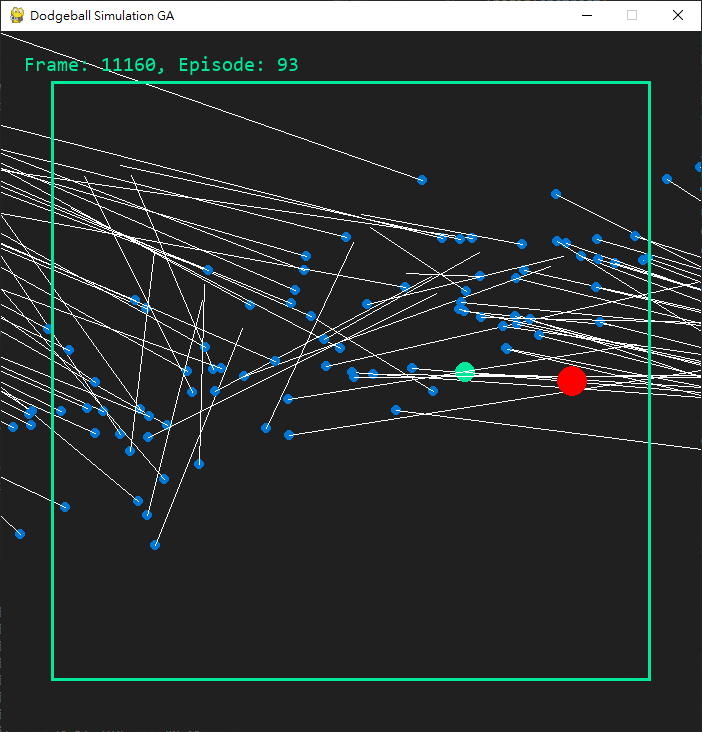
\includegraphics[width=0.9\linewidth]{imgs/demo01.png}
  \caption{The agents learning to pursue the target.}
  \Description{The agents learning to pursue the target.}
  \label{fig:ball_demo}
\end{figure}
As shown in \xfig{fig:ball_demo}, the simulation will include the following visible components:
\begin{itemize}
  \item \textbf{Game Arena:} A 2D field with a size $10\times10$ units, boundaries defined by a rectangle outlined in green.
  \item \textbf{Pursuing Agents:} AI agents, colored in blue, capable of moving in the 2D environment with the objective of pursuing the target. The one with the highest fitness value will be highlighted in green, while the one closest to the target will be highlighted in cyan.
  \item \textbf{Velocity indicator:} White line segments indicating the velocity vector of the agents, with the length of the line segment proportional to the magnitude of the velocity. This helps us visualize the direction and magnitude of the velocity of the agent.
  \item \textbf{Target Ball:} A simple ball, colored in red, with simulated physics, serving as the target for the pursuing agents. The target will be pushed at the beginning of each episode, moving in a straight line, and able to bounce off the boundaries of the game arena.
\end{itemize}

\subsection{Neural Network}
\begin{figure}[H]
  \centering
  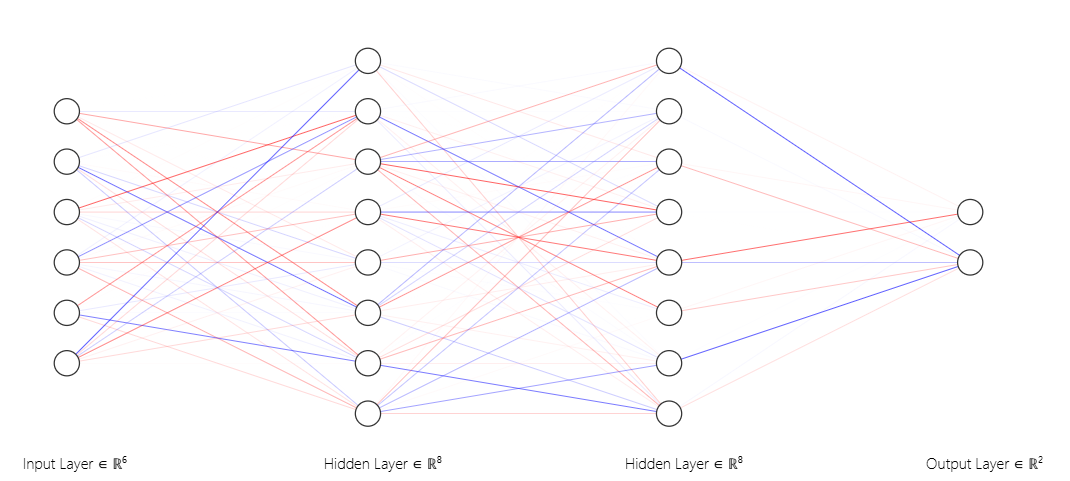
\includegraphics[width=0.9\linewidth]{imgs/NeuralNetwork.png}
  \caption{The structure of the neural network.}
  \Description{The structure of the neural network.}
  \label{fig:neural_network}
\end{figure}
The neural network architecture is fixed in this project and shown in \xfig{fig:neural_network}. It is a fully connected neural network implemented using Numpy library, consists of 4 layers: an input layer, two hidden layers, and an output layer. The input layer has 6 neurons, the two hidden layers have 8 neurons each, and the output layer has 2 neurons. The activation function used between layers is the hyperbolic tangent function (tanh). The neural network is initialized with Xavier initialization \label{imp_Initialization}\cite{Xavier_pmlr-v9-glorot10a}, sampled from a normal distribution with mean 0 and standard deviation $\sqrt{\frac{2}{n_{in} + n_{out}}}$, where $n_{in}$ and $n_{out}$ are the number of input and output neurons respectively. The input to the neural network consists of the following components:
\begin{enumerate}
  \item The position of the agent
  \item The position of the target
  \item The velocity of the target
\end{enumerate}
which are concatenated into a six-dimensional vector.
The output of the neural network is a two-dimensional vector, representing the velocity of the agent. 
Weight optimization is performed after each generation, rather than after each frame, to reduce the computational cost.
In the next section, we will describe the genetic algorithm used to optimize the 146 weights and biases of the neural network.

\subsection{Genetic Algorithm}
\subsubsection{Chromosome Design} The chromosome is a vector of real numbers representing the weights and biases of the neural network, flattened and represented as a 1D array of real numbers, the weights of the neural network are flattened and concatenated into a single vector. The weights will be clipped to a upper and lower bound after mutation and crossover to prevent gradient explosion and vanishing.

\subsubsection{Population Initialization} The population is initialized with a fixed size of 100, with the chromosomes representing the weights of the neural network, the detail can be found in~\ref{imp_Initialization}. 
\subsubsection{Selection} Tournament Selection with a tournament size of 6 is used, the best and second best chromosomes are selected as parents.
\subsubsection{Crossover} One-point crossover is used with a probability of $\mu_c = 0.85$, a random point is selected and the genes after the point are swapped between the two parents.
\subsubsection{Mutation} A modified version of uniform mutation is used with a probability of $\mu_m = 0.25$. Geometric distribution is used to determine expected number of genes to be mutated on average, which is 4\% of the total number of genes in the chromosome. The selected indices are then mutated by adding a random value sampled from a normal distribution with mean 0 and standard deviation 0.1. 

\subsubsection{Fitness Function}
The fitness function consists of the following components:
\begin{enumerate}
  \item \textbf{Distance to Target:} The squared distance between the agent and the target, normalized to the range $[-1, 0]$ where -1 is the furthest agent to the target.
  \item \textbf{Rank of Distance:} The rank of the distance to the target among all agents, normalized to the range $[0, 1]$ where 1 is the closest agent to the target.
  \item \textbf{Direction to Target:} The cosine similarity between the direction of the agent and the direction to the target. Only values greater than 0.8 are considered, it serves as a bonus reward for agents that are moving towards the target, so we chose to not normalize it.
\end{enumerate}
The fitness function is the sum of the above components, and it is being calculated and accumulated for each time step during the episode.
The accumulated reward is the actuall fitness function used to evaluate the performance and stability of the agents.
\subsection{Inspirations from Reinforcement Learning}
\begin{enumerate}
  \item \textbf{Curriculum Learning:} Curriculum learning is a training strategy in which the difficulty of the task is gradually increased during training. In this project, the speed of the target is gradually increased during the first 20\% of the generation, and then kept constant for the rest of the generation.
  \item \textbf{Accumulated Reward and Discount Factor:} The accumulated reward is used as the fitness function, which is the sum of the rewards at each time step. The accumulated reward is used to encourage the agent to reach the target as quickly as possible. On top of this, a discount factor $\gamma = 0.99$ is used to reduce the old rewards in the episode, the reward at time step $t$ is multiplied by $\gamma^t$. The accumulated reward is calculated as follows:
  \begin{equation}
    R_t = \sum_{i=t}^{T} \gamma^{i-t} r_i
    \label{eq:discount}
  \end{equation}
\end{enumerate}


\section{Experiment Results}
\subsection{Distance to Target}
\begin{figure*}[t]
  \centering
  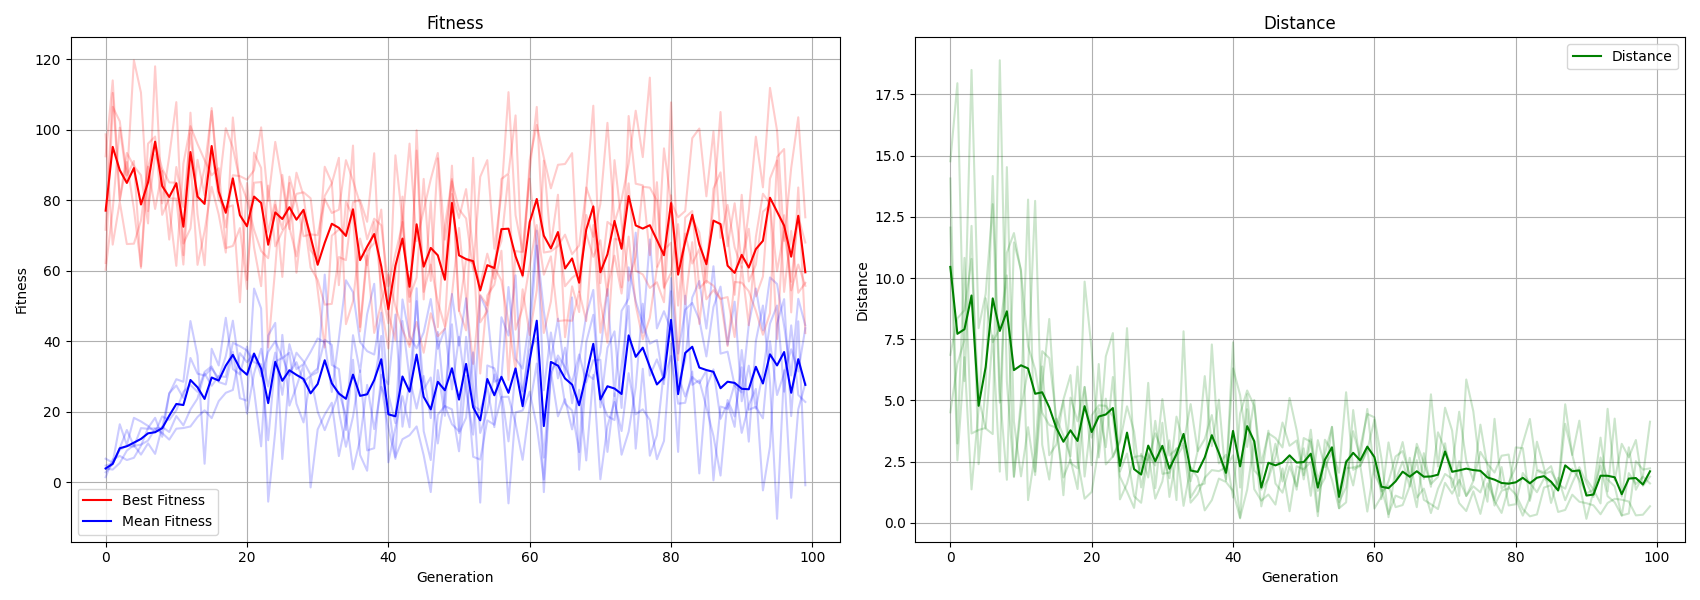
\includegraphics[width=0.95\linewidth]{imgs/result_Run_cx0.85_mut0.25_2024_1214_0619.png}
  \caption{The performance of the agents over the generations.}
  \Description{The performance of the agents over the generations.}
  \label{fig:plot_all}
\end{figure*}

\subsection{Fitness Function Analysis}
\begin{figure*}[t]
  \centering
  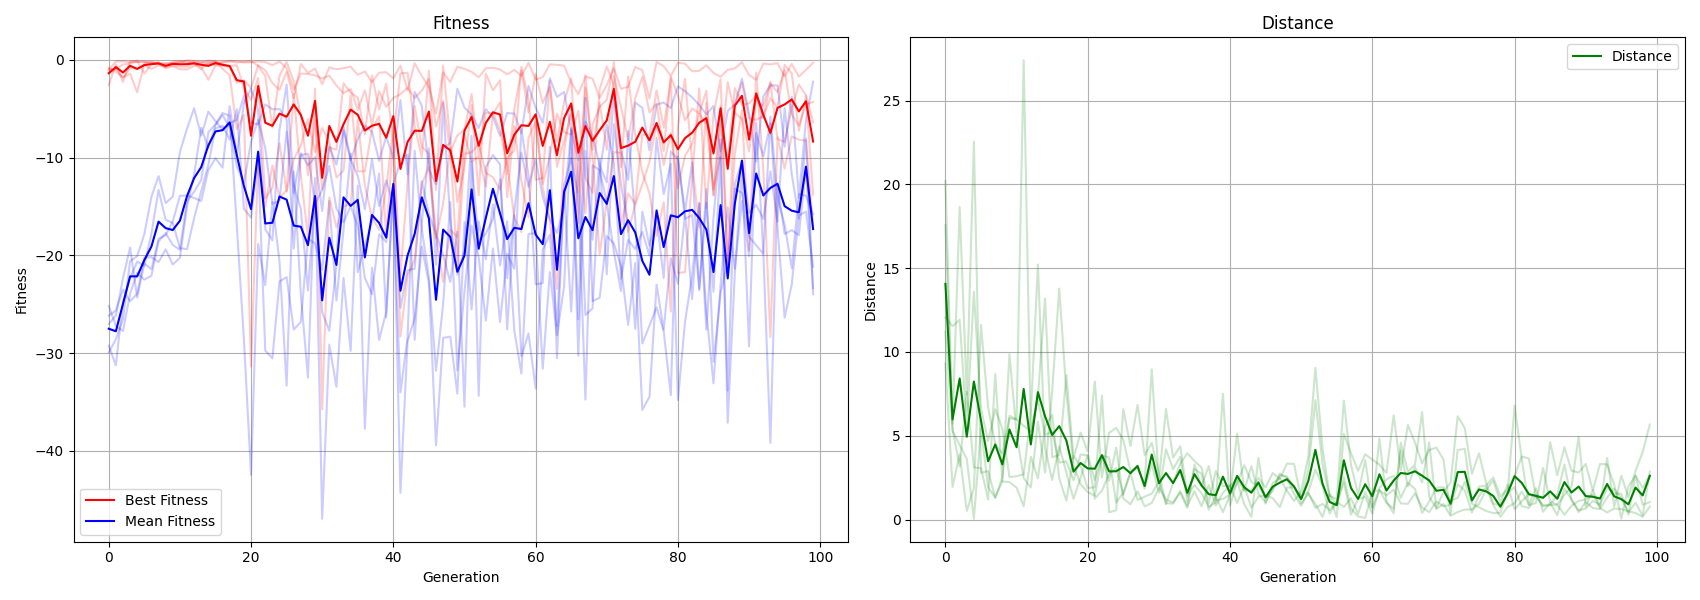
\includegraphics[width=0.95\linewidth]{imgs/result_Run_cx0.85_mut0.25_2024_1214_0633_dist_only.png}
  \caption{Using only the distance to target as the fitness function.}
  \Description{Using only the distance to target as the fitness function.}
  \label{fig:plot_dist}
\end{figure*}

\begin{figure*}[t]
  \centering
  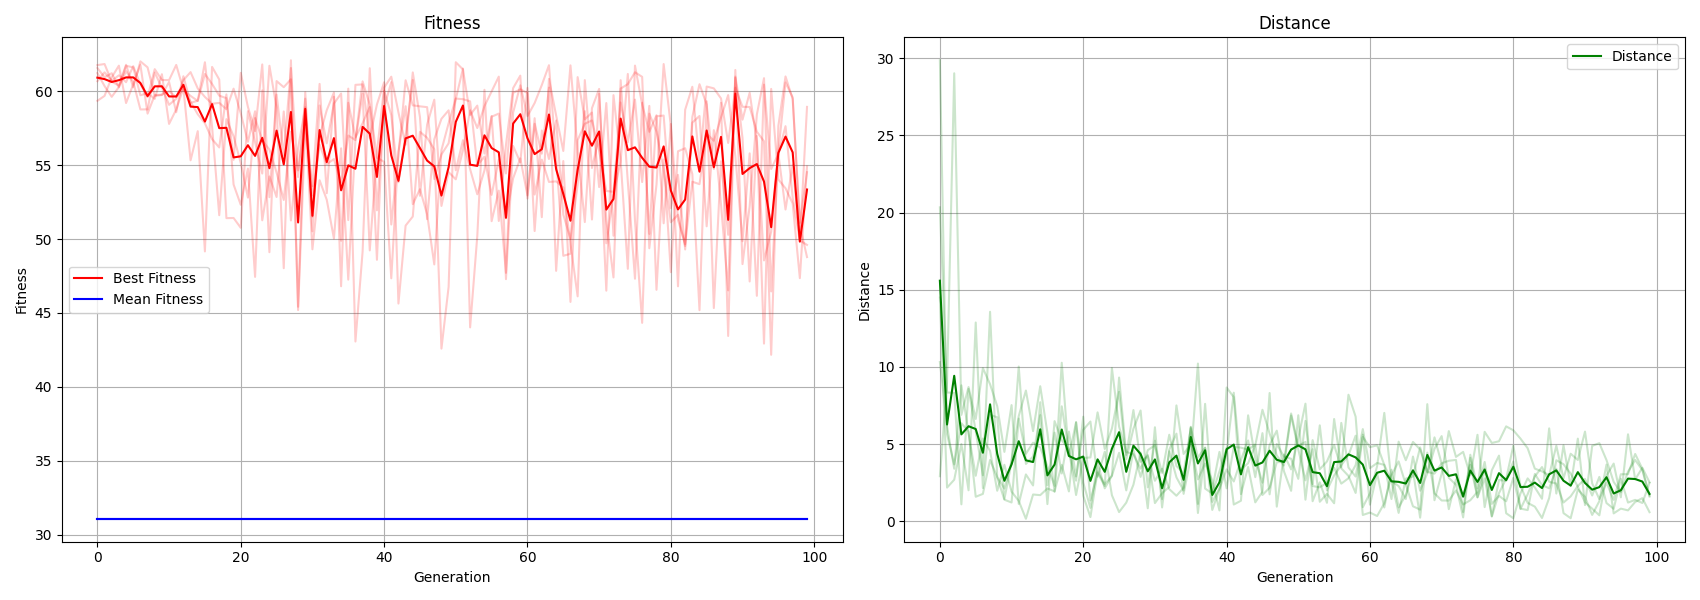
\includegraphics[width=0.95\linewidth]{imgs/result_Run_cx0.85_mut0.25_2024_1214_0634_rank_only.png}
  \caption{Using only the rank of distance as the fitness function.}
  \Description{Using only the rank of distance as the fitness function.}
  \label{fig:plot_rank}
\end{figure*}

\begin{figure*}[t]
  \centering
  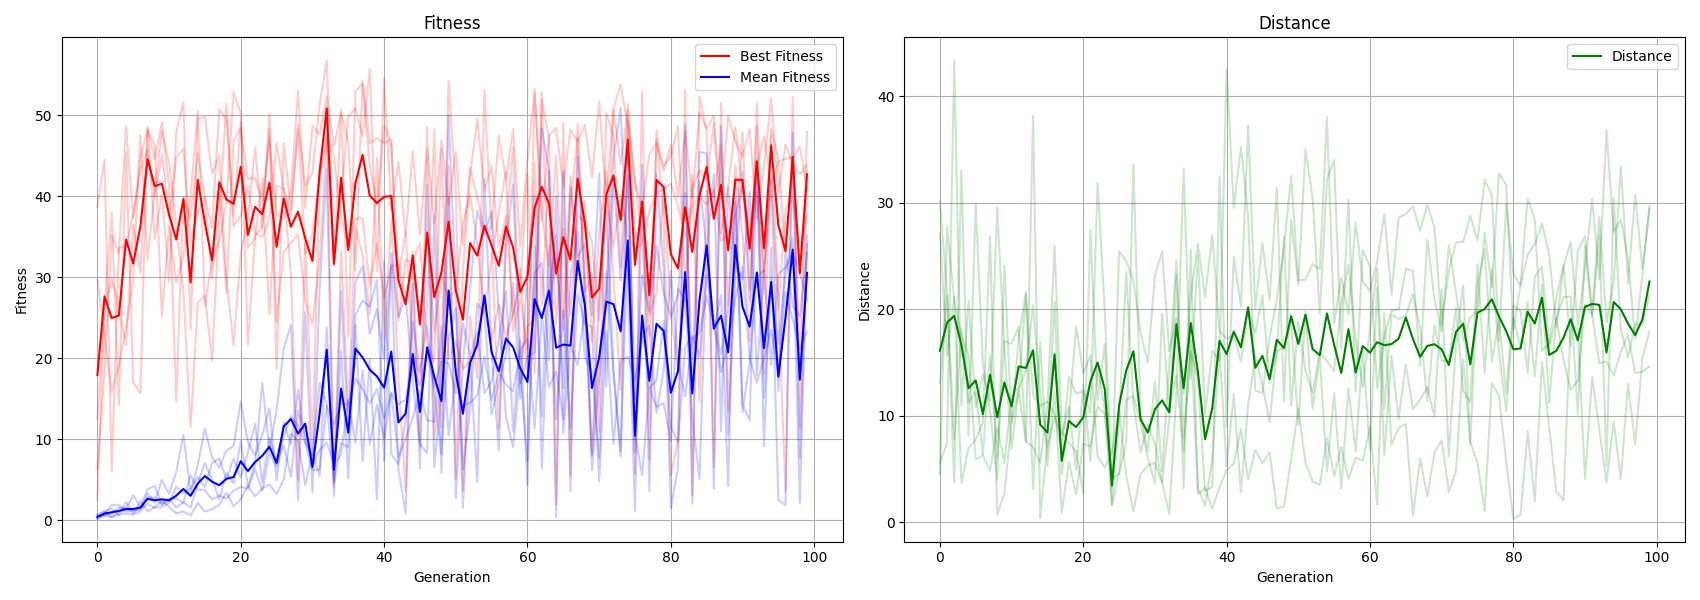
\includegraphics[width=0.95\linewidth]{imgs/result_Run_cx0.85_mut0.25_2024_1214_0636_dir_only.png}
  \caption{Using only the direction to target as the fitness function.}
  \Description{Using only the direction to target as the fitness function.}
  \label{fig:plot_dir}
\end{figure*}
\section{Conclusion}

\bibliographystyle{ACM-Reference-Format}
\bibliography{sample-base}

\end{document}
\endinput
%%
%% End of file `sample-sigconf.tex'.
